\documentclass[a4paper,11pt]{book}
%\documentclass[a4paper,twoside,11pt,titlepage]{book}
\usepackage{listings}
\usepackage[utf8]{inputenc}
\usepackage[spanish]{babel}

% \usepackage[style=list, number=none]{glossary} %
%\usepackage{titlesec}
%\usepackage{pailatino}

\decimalpoint
\usepackage{dcolumn}
\newcolumntype{.}{D{.}{\esperiod}{-1}}
\makeatletter
\addto\shorthandsspanish{\let\esperiod\es@period@code}
\makeatother


%\usepackage[chapter]{algorithm}
\RequirePackage{verbatim}
%\RequirePackage[Glenn]{fncychap}
\usepackage{fancyhdr}
\usepackage{graphicx}
\usepackage{afterpage}

\usepackage{float}

% Math style letters
\usepackage{amsfonts}
\usepackage{amsmath}

\usepackage{longtable}

\usepackage[pdfborder={000}]{hyperref} %referencia

% ********************************************************************
% Re-usable information
% ********************************************************************
\newcommand{\myTitle}{Biblioteca de algoritmos de detección de anomalías basados en técnicas de ensembles\xspace}
\newcommand{\myDegree}{Doble grado Ingeniería Informática y Matemáticas\xspace}
\newcommand{\myName}{Ignacio Aguilera Martos\xspace}
\newcommand{\myProf}{Francisco Herrera Triguero\xspace}
\newcommand{\myOtherProf}{Jacinto Carrasco Castillo\xspace}
%\newcommand{\mySupervisor}{Put name here\xspace}
\newcommand{\myFaculty}{Escuela Técnica Superior de Ingenierías Informática y de
Telecomunicación y Facultad de Ciencias\xspace}
\newcommand{\myFacultyShort}{E.T.S. de Ingenierías Informática y de
Telecomunicación y Facultad de Ciencias\xspace}
\newcommand{\myDepartment}{Departamento de Ciencias de la Computación e Inteligencia Artificial\xspace}
\newcommand{\myUni}{\protect{Universidad de Granada}\xspace}
\newcommand{\myLocation}{Granada\xspace}
\newcommand{\myTime}{\today\xspace}
\newcommand{\myVersion}{Version 0.1\xspace}


\hypersetup{
pdfauthor = {\myName (nacheteam@correo.ugr.es)},
pdftitle = {\myTitle},
pdfsubject = {},
pdfkeywords = {outlier, anomalía, ensemble},
pdfcreator = {LaTeX},
pdfproducer = {pdflatex}
}

%\hyphenation{}


%\usepackage{doxygen/doxygen}
%\usepackage{pdfpages}
\usepackage{url}
\usepackage{colortbl,longtable}
\usepackage[stable]{footmisc}
%\usepackage{index}

%\makeindex
%\usepackage[style=long, cols=2,border=plain,toc=true,number=none]{glossary}
% \makeglossary

% Definición de comandos que me son tiles:
%\renewcommand{\indexname}{Índice alfabético}
%\renewcommand{\glossaryname}{Glosario}

\pagestyle{fancy}
\fancyhf{}
\fancyhead[LO]{\leftmark}
\fancyhead[RE]{\rightmark}
\fancyhead[RO,LE]{\textbf{\thepage}}
\renewcommand{\chaptermark}[1]{\markboth{\textbf{#1}}{}}
\renewcommand{\sectionmark}[1]{\markright{\textbf{\thesection. #1}}}

\setlength{\headheight}{1.5\headheight}

\newcommand{\HRule}{\rule{\linewidth}{0.5mm}}
%Definimos los tipos teorema, ejemplo y definición podremos usar estos tipos
%simplemente poniendo \begin{teorema} \end{teorema} ...
\newtheorem{teorema}{Teorema}[chapter]
\newtheorem{proposicion}{Proposición}[chapter]
\newtheorem{ejemplo}{Ejemplo}[chapter]
\newtheorem{definicion}{Definición}[chapter]

\definecolor{gray97}{gray}{.97}
\definecolor{gray75}{gray}{.75}
\definecolor{gray45}{gray}{.45}
\definecolor{gray30}{gray}{.94}

\lstset{ frame=Ltb,
     framerule=0.5pt,
     aboveskip=0.5cm,
     framextopmargin=3pt,
     framexbottommargin=3pt,
     framexleftmargin=0.1cm,
     framesep=0pt,
     rulesep=.4pt,
     backgroundcolor=\color{gray97},
     rulesepcolor=\color{black},
     %
     stringstyle=\ttfamily,
     showstringspaces = false,
     basicstyle=\scriptsize\ttfamily,
     commentstyle=\color{gray45},
     keywordstyle=\bfseries,
     %
     numbers=left,
     numbersep=6pt,
     numberstyle=\tiny,
     numberfirstline = false,
     breaklines=true,
   }
 
% minimizar fragmentado de listados
\lstnewenvironment{listing}[1][]
   {\lstset{#1}\pagebreak[0]}{\pagebreak[0]}

\lstdefinestyle{CodigoC}
   {
	basicstyle=\scriptsize,
	frame=single,
	language=C,
	numbers=left
   }
\lstdefinestyle{CodigoC++}
   {
	basicstyle=\small,
	frame=single,
	backgroundcolor=\color{gray30},
	language=C++,
	numbers=left
   }

 
\lstdefinestyle{Consola}
   {basicstyle=\scriptsize\bf\ttfamily,
    backgroundcolor=\color{gray30},
    frame=single,
    numbers=none
   }


\newcommand{\bigrule}{\titlerule[0.5mm]}


%Para conseguir que en las páginas en blanco no ponga cabecerass
\makeatletter
\def\clearpage{%
  \ifvmode
    \ifnum \@dbltopnum =\m@ne
      \ifdim \pagetotal <\topskip
        \hbox{}
      \fi
    \fi
  \fi
  \newpage
  \thispagestyle{empty}
  \write\m@ne{}
  \vbox{}
  \penalty -\@Mi
}
\makeatother

\usepackage{pdfpages}
\begin{document}
\begin{titlepage}
 
 
\newlength{\centeroffset}
\setlength{\centeroffset}{-0.5\oddsidemargin}
\addtolength{\centeroffset}{0.5\evensidemargin}
\thispagestyle{empty}

\noindent\hspace*{\centeroffset}\begin{minipage}{\textwidth}

\centering

\includegraphics[width=0.9\textwidth]{imagenes/logo_ugr.jpg}\\[1.4cm]

\textsc{ \Large TRABAJO FIN DE GRADO\\[0.2cm]}
\textsc{ INGENIERÍA EN ...}\\[1cm]
% Upper part of the page
% 
% Title
{\Huge\bfseries Titulo del Proyecto\\
}
\noindent\rule[-1ex]{\textwidth}{3pt}\\[3.5ex]
{\large\bfseries Subtitulo del Proyecto}
\end{minipage}

\vspace{2.5cm}
\noindent\hspace*{\centeroffset}\begin{minipage}{\textwidth}
\centering

\textbf{Autor}\\ {Nombre Apellido1 Apellido2 (alumno)}\\[2.5ex]
\textbf{Directores}\\
{Nombre Apellido1 Apellido2 (tutor1)\\
Nombre Apellido1 Apellido2 (tutor2)}\\[2cm]

\includegraphics[width=0.3\textwidth]{imagenes/etsiit_logo.png}\\[0.1cm]
\textsc{Escuela Técnica Superior de Ingenierías Informática y de Telecomunicación}\\
\textsc{---}\\
Granada, mes de 201
\end{minipage}
%\addtolength{\textwidth}{\centeroffset}
%\vspace{\stretch{2}}
\end{titlepage}



\chapter*{}
%\thispagestyle{empty}
%\cleardoublepage

%\thispagestyle{empty}

\begin{titlepage}
 
 
\setlength{\centeroffset}{-0.5\oddsidemargin}
\addtolength{\centeroffset}{0.5\evensidemargin}
\thispagestyle{empty}

\noindent\hspace*{\centeroffset}\begin{minipage}{\textwidth}

\centering
%
\includegraphics[width=0.9\textwidth]{imagenes/logo_ugr.jpg}\\[1.4cm]

%\textsc{ \Large PROYECTO FIN DE CARRERA\\[0.2cm]}
%\textsc{ INGENIERÍA EN INFORMÁTICA}\\[1cm]
% Upper part of the page
% 

 \vspace{3.3cm}

%si el proyecto tiene logo poner aquí
%
\includegraphics{imagenes/logo.png} 
% \vspace{0.5cm}

% Title

{\Huge\bfseries Detección de anomalías basada en técnicas de ensembles\\
}
\noindent\rule[-1ex]{\textwidth}{3pt}\\[3.5ex]
{\large\bfseries Biblioteca de algoritmos\\[4cm]}
\end{minipage}

\vspace{2.5cm}
\noindent\hspace*{\centeroffset}\begin{minipage}{\textwidth}
\centering

\textbf{Autor}\\ {Ignacio Aguilera Martos}\\[2.5ex]
\textbf{Directores}\\
{Francisco Herrera Triguero}\\[2cm]
%
\includegraphics[width=0.15\textwidth]{imagenes/tstc.png}\\[0.1cm]
%\textsc{Departamento de Teoría de la Señal, Telemática y Comunicaciones}\\
%\textsc{---}\\
%Granada, mes de 201
\end{minipage}
%\addtolength{\textwidth}{\centeroffset}
\vspace{\stretch{2}}

 
\end{titlepage}






\cleardoublepage
\thispagestyle{empty}

\begin{center}
{\large\bfseries Detección de anomalías basada en técnicas de ensembles: Biblioteca de algoritmos}\\
\end{center}
\begin{center}
Ignacio Aguilera Martos\\
\end{center}

%\vspace{0.7cm}
\noindent{\textbf{Palabras clave}: anomalía, ensamblaje, python, hics, outres, loda, mahalanobis kernel, trinity, aprendizaje automático, estadística}\\

\vspace{0.7cm}
\noindent{\textbf{Resumen}}\\

La detección de anomalías es un ámbito de estudio que está ganando relevancia por ser una parte interesante en el tratamiento de los datos. Actualmente hacemos un manejo y un uso de los datos cada vez más voraz y creciente, necesitando no sólo técnicas que nos permitan obtener información de ellos sino además preprocesamiento de los datos que haga que estas técnicas funcionen de forma más eficiente. 

Las anomalías no sólo son útiles en el preprocesamiento de los datos, también son interesantes en detección de eventos atípicos en los mismos. Por ejemplo, podemos aplicar esta detección en casos como detección de fraude en compras con tarjetas bancarias o por ejemplo en predicción de fallos en sistemas como los frenos de un coche o un camión.

Para ello en el trabajo haremos un breve repaso de cuáles son las herramientas teóricas que hacen que el trabajo de nuestros algoritmos y modelos sea consistente y funcione así como herramientas estadísticas y del ámbito de la probabilidad que explican el funcionamiento de alguno de los modelos. 

Finalmente el trabajo desembocará en la implementación de algunos de los modelos del estado del arte en el ámbito de la detección de anomalías y su comparativa con modelos considerados como clásicos o tradicionales. Es decir, pondremos en contraposición los modelos de ensamblaje con los tradicionales para estudiarlos comparativamente. Asimismo veremos algunas conclusiones sobre los modelos y una propuesta de trabajo futuro con la intención de mejorar la situación actual de los modelos de ensamblaje.

\cleardoublepage


\thispagestyle{empty}


\begin{center}
{\large\bfseries Outlier detection based in ensemble methods: Library implementation}\\
\end{center}
\begin{center}
Ignacio Aguilera Martos\\
\end{center}

%\vspace{0.7cm}
\noindent{\textbf{Keywords}: outlier, ensemble, python, hics, outres, loda, mahalanobis kernel, trinity, machine learning, statistics}\\

\vspace{0.7cm}
\noindent{\textbf{Abstract}}\\

Nowadays it's being more and more important the analysis of outliers in the area of data preprocessing. The way we are using the data is more and more greedy and we need better ways of mining the knowledge from the data. The use of outlier detection can lead to better performance of the Machine Learning models as we can now detect the outliers and eliminate them or treat them separately. Another approach is the detection of certain events due to the appearance of outliers. For example we can have a record of a certain bank and the credit card users. If someone gets his card stolen the way the thief buys and where the payments occur can lead to a detection of an anomalous way of using this card and therefore to inform the person that he could have his card stolen.

The anomaly detection could be useful as well in various field as medicine or event detection. We could think and measure the failure of the brake system of a truck or an earthquake as an anomaly in our datasets and we could detect them or event predict them.

The aim of this project is the discussion of ensemble models against the conventional ones in the discussion of the dilema of meta-algorithms versus simple algorithms. This study accomplishes the task of theoretical and practical discussion of the topic as well as further conclusions towards future work.

The way we introduced the outlier detection and study on this job has been preceded by a deep study on Machine Learning and the statistics it envolves. This previous study is due to the importance of understanding why the algorithms and models implemented in this job are suitable for their use and therefore we can know as well their limits. This section has a description and introduction of the Machine Learning area and it evolves on the study of ERM and the in sample and out sample dilema in the field.

After this study the first concept of outlier is given based on distances and quartiles. It is not only important the way we define the outliers but also why should we consider detecting them on our datasets before getting any further work done. Criterions and possibilities are described in this section. 

Probability, and even more multivariate probability, is very important in our study. Nearly all models implemented base their working principple on density or probability estimation. For this reason I've considered getting our hands firs on a multivariate introduction with useful concepts for explaining and understanding the model. This does not means that all concepts are going to be used in the study but, those included have been useful to me in the process of understanding how the theory of the models is built around. 

Due to this probability introduction a new outlier definition is available to us through these concepts. A probability-based definition of outlier is given and then used in serveral models as HICS or OUTRES. This probability definition involves probability density expectation, marginal distribution and joint distribution. This definition is not put against the distance based one, but to complement of fullfill the first definition with non trivial outliers.

All this theory gives us way to approach the model implementation. The concept of ensemble appears here as the algorithms used in this study are no conventional ones. As the title says, the study goes around outlier ensembles. The concept is given here as the final goal is to make a reasonable comparison between the outlier detection algorithms, those called ensembles and what we could consider as traditional or conventional. 

This portfolio contains the implementation and explanation of the five models chosen: HICS, OUTRES, Trinity, Mahalanobis Kernel and LODA. They are not chosen by coincidence but trying to cover most of the types of algorithms avaiable in the state of art of outlier ensembles. HICS and OUTRES are from the subtype of ensembles called subspace miners of subspace based. The basic explanation of them is that they try to analyze the data in certain subspaces so they can measure the density in each one of them and compare it to the rest of the instances of the dataset. HICS mantaing the point of view of choosing the subspaces with no relation or conection with the instances of the dataset while OUTRES tries the other way around, this is choosing the subspace based on the instance we are considering. Mahalanobis Kernel is a PCA-based algorithm or at leats PCA-influenced as it belongs to the same category. Trinity is a meta-model or meta-algorithm, this is a algorithm that combines simple models in order to obtain a more robust algorithm. Finally LODA uses the last technique I've chosen which is histogram-based. The short explanation of this type of model is the use of histograms to study the frequency of appearance of a certain data of value.

So now we have all set up for our experiments. For the implementation Python has been chosen for several reasons. First of all Python is a versatile flexible language giving a lot of possibilities on the libraries you can use. Second we can make the development usefull for more people as Python is one of the most used languages on data science. For this reason I've decided to make myself a library with the algorithms implemented so they can be easily used by Python users and furthermore the development is completely open and available in GitHub so that anyone can see the code, understand it and fix bugs or extend the library content with new models if necessary.

All models are put against the same set of datasets given from the Stony Brooks University. This University mantains a set of datasets for outlier detection with the ground truth available so practitioners can work with it. These datasets allow us to treat the problem as a semi-supervised problem as we can obtain at the end a percentage of accuracy. The work first executes all models on these datasets to measure the performance of the ensemble models. To compare them with the classical ones we need the implementation of those classical. For this purpose the library PyOD is used. This library contains the implementation of a lot of models including some ensemble algorithms but not the ones I've chosen. With these implementations we can compare the accuracy and times of the models over the datasets. For a better understanding of the models they are analyzed individually if necessary.

So, I have ended up with a study of the state of art of ensemble algorithms putting them against the classical approach to see who outperforms whom. Future work is also discused at the end of this portfolio as the possibilities of improvement are still there due to the difficulty of the problem.

\chapter*{Agradecimientos}
\thispagestyle{empty}

       \vspace{1cm}


Poner aquí agradecimientos...


\frontmatter
\tableofcontents
%\listoffigures
%\listoftables
%
\mainmatter
\setlength{\parskip}{10pt}

\chapter{Introducción}

Antes de comenzar el objeto de estudio de este trabajo, lo primero que debemos hacer es contextualizar el mismo y establecer un marco de trabajo en cuanto a teoría que se empleará en la posterior experimentación y desarrollo del mismo. 

El estudio realizado y plasmado en este trabajo se centra en la obtención de técnicas para la detección de anomalías en conjuntos de datos, concepto que introduciremos posteriormente. En concreto las técnicas que se van a desarrollar son las conocidas como técnicas de ensemble que se basan en el estudio del problema o bien combinando modelos existentes o bien haciendo un estudio pormenorizado aplicando algún criterio por subespacios del conjunto de datos. 

En primer lugar el trabajo desarrollará una introducción a la teoría de aprendizaje y resolución de problemas mediante datos y no por diseño así como la teoría matemática que esto involucra. Esta primera sección nos dará suficiente estructura al trabajo para poder definir en términos de distancias lo que significa que una instancia de un conjunto de datos sea una anomalía.

Posteriormente se desarrollará brevemente algunos conocimientos estadísticos básicos de estadística multivariante para poder introducir el concepto de anomalía desde la perspectiva de las probabilidades condicionadas.

Tras esto podremos entrar en el terreno de la experimentación, desarrollo y explicación de técnicas y puesta en contraste con los algoritmos clásicos para comprobar el desempeño de las nuevas técnicas.

Por último se presentarán las conclusiones obtenidas tras todo este estudio.
%
\part{Machine Learning y el concepto de Anomalía}
\label{part:machineLearning_anomalia}

En esta sección vamos a centrarnos en dos aspectos: el Machine Learning para establecer las herramientas usadas en el estudio y el propio concepto de anomalía y algunas reflexiones acerca del mismo.

\chapter{Machine Learning}
\label{chapter:machine_learning}

En este capítulo vamos a hacer un repaso sobre los conceptos asociados al Machine Learning, el aprendizaje y la teoría matemática que involucra. Estas herramientas y conceptos los utilizaremos posteriormente para resolver el problema de detección de anomalías.

\section{Contextualización del aprendizaje}

Para comenzar tenemos que empezar definiendo en que consiste el proceso de aprender sobre unos datos. Supongamos que tenemos un problema en el que tenemos una entrada y una salida, por ejemplo una entrada válida podría ser un vector $x\in \mathbb{R}^d$ y una salida un valor real o un número natural. El problema de aprendizaje intenta estimar una estructura de tipo entrada-salida como la descrita usando únicamente un número finito de observaciones.

Podemos definirlo de forma más general empleando tres conceptos:

\begin{itemize}
	\item Generador: El generador se encarga de obtener las entradas $x\in \mathbb{R}^d$ mediante una distribución de probabilidad $p(x)$ desconocida y fijada de antemano.
	\item Sistema: El sistema es el que produce la salida ``y'' (correcta) para cada entrada $x\in \mathbb{R}^d$ mediante la distribución de probabilidad $p(x|y)$ desconocida y fijada de antemano.
	\item Máquina de aprendizaje: esta es la que va a obtener información de las entradas y salidas conocidas para intentar predecir la salida correcta para una entrada nueva que se nos de. De forma abstracta esta máquina lo que hace es tomar una serie de funciones de un conjunto general de forma que para una entrada dada $x$ la función $f(x,\omega)$ con $\omega \in \Omega$ nos de la salida que corresponde para $x$ donde $\omega$ es una forma de indexar las funciones tomadas para generalizar la salida del conjunto más general de funciones que hemos indicado.
\end{itemize}

El único cabo que hemos dejado sin atar en las definiciones que acabamos de ver es el conjunto de funciones del cual tomaremos algunas para adaptar la máquina de aprendizaje a los datos recibidos. Este conjunto de funciones, que notaremos como $\mathcal{H}$, es de momento la única forma que tenemos de aplicar un conocimiento a priori en la máquina de aprendizaje.

Para finalizar esta breve introducción y poder continuar profundizando vamos a exponer algunos ejemplos de clases de funciones para que podamos visualizar el contexto.

\begin{itemize}
	\item Funciones lineales: En este caso la clase de funciones $\mathcal{H}$ está formada por funciones de la forma $h(x) = w_0 + \sum_{i=1}^{d}x_i w_i$ donde $w\in \mathbb{R}^{d+1}$. Este es el modelo de funciones más clásico.
	\item Funciones trigonométricas: Un ejemplo de una clase de funciones trigonométricas podría ser $f_m(x,v_m,w_m) = \sum_{j=1}^{m-1}(v_j \sin (jx) + w_j \cos (jx)) + w_0$ donde en este caso la entrada es un único valor real. Este tipo de clases de funciones serán útiles en problemas de regresión que luego explicaremos con algo más de detalle aunque sin centrarnos mucho en ello pues no es el objetivo del estudio.
\end{itemize}

\subsection{Objetivo del aprendizaje}

Cuando hablamos de aprendizaje queremos obtener algo de dicho aprendizaje a partir de los datos. Como ya se ha mencionado, intentamos obtener una función de una familia de funciones que aproxime o modele de buena manera la salida del sistema. Por tanto, ese es nuestro objetivo: obtener una función de la familia de funciones que minimice el error.

El problema que enfrentamos es que sólo disponemos de un número finito, por ejemplo $n$, de observaciones de datos y su correspondiente salida. Esto nos va a hacer que no podamos tener una garantía de optimalidad a no ser que tendamos $n$ a infinito. 

Sin embargo si que podemos cuantificar cómo de buena es una aproximación con respecto a otra mediante la función pérdida o error que denotaremos como $L(y,f(x,\omega))$. Esta función nos va a medir la diferencia entre la salida real del sistema y la salida dada por la función $f$ para la entrada $x$ siendo siempre $L(y,f(x,\omega))\geq 0$.

Recordemos además que el Generador obtiene datos mediante una distribución desconocida pero fijada de antemano y que son independientes e idénticamente distribuidos con respecto a la distribución conjunta, es decir:

$$p(x,y) = p(x)p(y|x)$$

Una vez definido todo esto podemos obtener el valor esperado de pérdida o error mediante el funcional

$$R(\omega) = \int L(y,f(x,\omega))p(x,y)dxdy$$

Ahora podemos concretar un poco más lo que entendemos como objetivo del aprendizaje. El objetivo será encontrar una función $f\in \mathcal{H}$ que nos minimice el valor del funcional $R(\omega)$. Pero recordemos que $p(x,y)$ es desconocida para nosotros, por lo que no podemos saber cómo se distribuyen los datos y por tanto el valor del funcional no es calculable para nosotros y por tanto la solución puramente de cálculo no es accesible.

Por tanto, la única forma realmente potente y útil de encontrar una buena aproximación será incorporar el conocimiento a priori que tenemos del sistema. En la sección anterior hemos visto que una forma de incorporar dicho conocimiento es mediante la selección de la clase de funciones, pero además será muy relevante el hecho de cómo los datos son empleados en el proceso de aprendizaje. En este apartado de decisión tendremos que resolver primero la codificación de los datos, el algoritmo empleado y el uso de técnicas como la regularización que veremos después para incorporar nuestro conocimiento en el camino que nos lleve a la solución.

\subsection{Clases de aprendizaje}

El problema de aprendizaje puede ser subdividido a su vez en cuatro clases distintas y que se suelen abordar de forma independiente. Estoss tipos de problemas de aprendizaje son:

\begin{itemize}
	\item Clasificación: El problema de clasificación consiste en identificar y separar instancias de datos según su clase. Por ejemplo podemos dividir a la población mundial en dos clases: sanos y enfermos. Un problema de clasificación podría ser saber identificar estas clases para un conjunto de personas. Los problemas de clasificación más sencillos son aquellos en los que se usan dos únicas clases aunque se puede generalizar la definición del problema a k-clases.
	\item Regresión: El problema de regresión consiste en estimar una función $f: \mathbb{R}^n \rightarrow \mathbb{R}$ a partir de una serie de muestras previas con los valores de $f$. Un problema de regresión podría ser determinar la función que, dados los datos de altura y dimensiones corporales sea capaz de darnos el peso aproximado de la persona.
	\item Estimación de la función de densidad: en este caso no nos interesa la salida que proporciona el sistema, ya sea el valor de una clase o una función real como en el caso de la regresión. En este caso el objetivo del aprendizaje es conseguir la función de densidad $f(x,\omega)$, con $\omega \in \Omega$ los parámetros necesarios de la función de densidad, con la que se distribuyen los datos de entrada del sistema.
	\item Agrupamiento y cuantificación vectorial: El problema de cuantificación vectorial consiste en intentar explicar la distribución de los vectores de entrada mediante puntos clave llamados centroides. De esta forma se podría reducir la complejidad de los datos expresándolos en función de un sistema de generadores menor. El problema de agrupamiento tiene también relación por utilizar la idea de centroide, pero el objetivo es completamente distinto. El objetivo del problema de agrupamiento es intentar conseguir agrupar los datos en clusters, es decir, regiones del espacio en las que se concentran un conjunto de datos. De esta forma intentamos agrupar los datos que mantienen una relación entre sí. Un ejemplo de un problema de cuantificación vectorial podría ser un problema de reducción de dimensionalidad y un ejemplo de problema de agrupamiento podría ser identificar instancias de datos con características comunes.
\end{itemize}

\section{Principios y adaptación del aprendizaje}

Según Vapnik \cite{vapnik_v._nature_nodate} la predicción mediante el aprendizaje se puede dividir en dos fases:

\begin{enumerate}
	\item Aprendizaje o estimación a partir de una muestra.
	\item Predicción a partir de las estimaciones obtenidas.
\end{enumerate}

Estas dos fases se corresponden con los dos tipos de inferencia clásica que conocemos, esto es, inducción y deducción. Traído a este caso el proceso de inducción es aquel que a partir de los datos de aprendizaje o los datos de la muestra que tenemos con la salida que corresponde podemos estimar un modelo. Es decir, estamos sacando el conocimiento de los datos para generar el modelo. El proceso de deducción es aquel que, una vez obtenido el modelo estimado (la generalización) obtenemos una predicción de la salida sobre un conjunto de datos.

Por contra, Vapnik propone un paso que resuelve estas dos fases directamente y que él denomina transducción. Este paso consiste en, dados los datos de entrenamiento obtenemos directamente los valores de salida sin tener que hacer la generalización a un modelo. De esta forma, según Vapnik, podríamos reducir el error que cometemos en la predicción. Este razonamiento tiene sentido, pues estamos omitiendo el paso más complejo del proceso de inducción-deducción.

En resumen esta idea se puede resumir en la siguiente figura:

\begin{figure}[H]
	\centering
	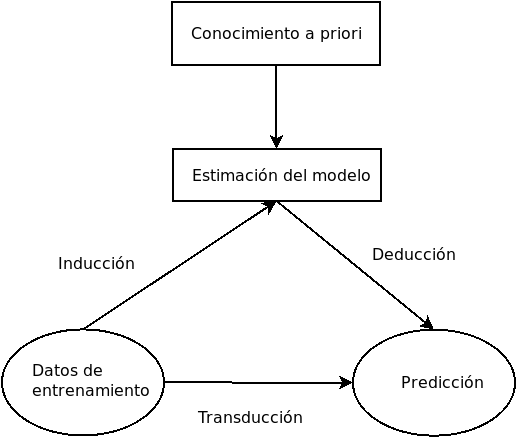
\includegraphics[scale=0.5]{imagenes/induccion_deduccion_transduccion}
	\label{ind_ded_trans}
	\caption{Tipos de inferencia y transduccion \cite[p.~41]{cherkassky_learning_2007}}
\end{figure}

Podemos ver que el conocimiento a priori que tenemos del problema se manifiesta una vez se crea el modelo general, de forma que se emplearía en el paso de la inducción. Ya hemos hablado previamente del conocimiento a priori y cómo incorporarlo al modelo, pero por concretar un poco más podemos añadirlo básicamente de dos formas:

\begin{itemize}
	\item Escogiendo un conjunto de funciones para aproximar la salida del sistema
	\item Añadiendo restricciones o penalizaciones adicionales a dicho conjunto de funciones.
\end{itemize}

En resumen, para poder crear la generalización del modelo de forma única necesitamos:

\begin{enumerate}
	\item Un conjunto de funciones para aproximar la salida.
	\item Conocimiento a priori.
	\item Un principio inductivo, que no es más que una indicación de cómo emplear los datos para llegar a la generalización del modelo.
	\item Un método de aprendizaje, es decir, una implementación del principio inductivo.
\end{enumerate}

En secciones posteriores revisaremos algunos de los principios inductivos más usados pero es importante reseñar la diferencia entre pricipio inductivo y método de aprendizaje. Para un mismo principio inductivo podemos tener varios métodos de aprendizaje, pues podemos escoger diferentes formas de llevarlo a la práctica. Por ejemplo, uno de los principios inductivos más empleados es el ERM o Empirical Risk Minimization, es decir, minimización del error empírico. Podríamos pensar en diferentes formas de utilizar este principio, por ejemplo sólo avanzamos en la creación del modelo si a cada paso que demos minimizamos el error, o por ejemplo vamos avanzando varios modelos a la vez hasta obtener un número de modelos finales de entre los cuales escogeremos aquel que mejor minimice dicho error.

\subsection{Principios inductivos}

Una vez introducido el concepto como hemos hecho en la sección anterior vamos a hacer un breve repaso de los principios más usados y en qué consiste cada uno de ellos.

\subsubsection{Penalización o Regularización}

Imaginemos que tenemos una clase de funciones muy flexible, esto es con un gran número de parámetros libres $f(x,\omega)$ con $\omega \in \Omega$. Vamos a partir de la base del ERM, es decir, minimizar el error empírico. La penalización lo que va a hacer es añadir un factor a la función a minimizar:

$$R_{pen}(\omega) = R_{emp}(\omega) + \lambda \phi [f(x,\omega)]$$

Donde $R_{emp}(\omega)$ es el error empírico con los parámetros $\omega$ y $\phi [f(x,\omega)]$ es un funcional no negativo asociado a cada estimación $f(x,\omega)$. El parámetro $\lambda >0$ es un escalar que controla el peso de la penalización.

El funcional $\phi [f(x,\omega)]$ puede medir lo que creamos conveniente que debemos añadir, es decir, aquí podemos añadir a la minimización algún tipo de medida que nos diga cómo de bien funciona el ajuste de los datos y cómo de bien funciona la información a priori que hemos incluido en el modelo. Pensemos por ejemplo que $\lambda$ fuera un parámetro con un valor muy alto. En este caso la penalización por un mal ajuste de los datos no sería de gran importancia pues lo más conveniente sería minimizar el valor del funcional para no obtener una gran penalización. De esta forma podemos ajustar y dar un poco más de información al error empírico. Por ejemplo, en función del problema, es posible medir la complejidad de la solución mediante el funcional $\phi$ y de esta forma no sólo vamos a obtener una función que ajuste bien los datos, si no que también mantenga una cierta simplicidad para evitar por ejemplo el sobreajuste.

\subsubsection{Reglas de parada anticipada}

Pensemos en un método que vaya aprendiendo de los datos de forma iterativa intentando a cada iteración reducir el error cometido, por ejemplo el ERM. Los métodos o reglas de parada anticipada pueden verse como penalizaciones sobre el algoritmo conforme se va ejecutando. Las reglas de parada anticipada, como su nombre indica lo que preveen es la parada del algoritmo antes de obtener su objetivo teórico. Por ejemplo un algoritmo intenta que el error sea menor que $10^{-6}$ pero para reducirlo desde $10^{-4}$ hasta $10^{-5}$ está consumiendo millones de iteraciones. Si queremos que el tiempo de cómputo penalice lo que podemos hacer es fijar por ejemplo un número máximo de iteraciones que detenga el método aunque no se haya alcanzado esa barrera de error que se preveía.

\subsubsection{Minimización del riesgo estructural o SRM}

Para entender esta filosofía nos ponemos en la situación de que ya sabemos la clase de funciones con la que vamos a aproximar la salida del sistema, por ejemplo hemos escogido la clase de funciones polinómicas. Bajo esta clase de funciones podemos ordenar las funciones por complejidad, entendiendo por complejidad el número de parámetros de la función. Por ejemplo los polinomios de grado $m$ son de menor complejidad que los de grado $m+1$. De esta forma podemos pensar en una estructura de la clase de funciones de la forma:

$$S_0 \subset S_1 \subset S_2 \subset \cdots$$

Este parámetro de complejidad también puede ser un principio a minimizar para intentar conseguir una solución adecuada pero también simple. La generalización de la medida de complejidad para las clases de funciones es la conocida como dimensión VC o dimensión de Vapnik-Chervonenkis.

\subsubsection{Inferencia Bayesiana}

Este principio inductivo se utiliza en el problema de estimación de la función de densidad. El principio es utilizar la conocida fórmula de Bayes para hacer una estimación de la función de densidad empleando el conocimiento a priori que disponemos del problema. La forma en la que se emplea esta fórmula es de la siguiente:

$$P[modelo | datos] = \frac{P[datos | modelo] \cdot P[modelo]}{P[datos]}$$

donde $P[modelo]$ es la probabilidad a priori, $P[datos]$ es la probabilidad de los datos de entrenamiento y $P[datos | modelo]$ es la probabilidad de que los datos estén generados por el modelo.

\subsubsection{Descripción de mínima longitud}

La idea de este principio es la minimización de la longitud que se necesita emplear para describir un modelo y la correspondiente salida. Llamamos l a la longitud total:

$$l = L(modelo) + L(datos | modelo)$$

Esta medida puede ser vista como una medida de complejidad conjunta de todo el modelo.

\section{Regularización}

Por la importancia de este principio inductivo vamos a desarrollarlo un poco más, junto con el concepto de penalización, la selección de los modelos y la relación entre sesgo y varianza. Este último es un concepto muy relevante en cuanto al aprendizaje y que en nuestro caso, al no poseer la clasificación real tendremos que tenerlo en cuenta.

\subsection{Problema de la alta dimensionalidad}

Sabemos que cuando estamos ante un problema de aprendizaje nuestro objetivo es conseguir estimar una función con un número finito de instancias de una muestra ya con la salida. Al tener un número finito de elementos en la muestra ya sabemos que no podemos garantizar que la respuesta sea la óptima o correcta, pero además debemos pensar que a mayor regularidad del conjunto de funciones empleado debemos tener una densidad suficiente de puntos para compensar dicha regularidad. Este problema es conocido como la maldición de la dimensionalidad (curse of dimensionality). El problema es que cuanto mayor sea la dimensionalidad considerada más difícil es poder tener esa alta densidad de datos que se requieren para funciones muy regulares.

Este problema que conlleva la alta dimensionalidad proviene de la geometría de los espacio con alta dimensionalidad. A medida que incrementamos la dimensionalidad el espacio se ve cada vez con más aristas o picos. Podemos pensar en un cubo para el espacio tridimensional y a medida que aumentamos la dimensión incorporamos más aristas y vértices. Podemos resumir en 4 propiedades de los espacio con alta dimensionalidad que causan este problema:

\begin{enumerate}
	\item La densidad disminuye exponencialmente al aumentar el número de dimensiones. Supongamos que tenemos una muestra de $n$ puntos en $\mathbb{R}$. Para poder tener la misma densidad en un espacio $d$-dimensional $\mathbb{R}^d$ necesidamos $n^d$ puntos.
	\item Cuanto mayor dimensionalidad tenga el conjunto de datos mayor lado se necesita para que un hipercubo contenga el mismo porcentaje del conjunto que con una menor dimensionalidad. Imaginemos que tenemos un conjunto $d$-dimensional en el que tenemos la muestra dentro de un hipercubo unidad. Si quisiéramos abarcar un porcentaje $p\in [0,1]$ necesitaríamos un cubo de lado $e_d (p) = p^{\frac{1}{d}}$. Como se puede observar a mayor dimensionalidad y $p$ constante el lado es cada vez mayor. Esta idea es fácilemente entendible si observamos la siguiente figura:
	
	\begin{figure}[H]
		\centering
		\label{radio_alta_dimensionalidad}
		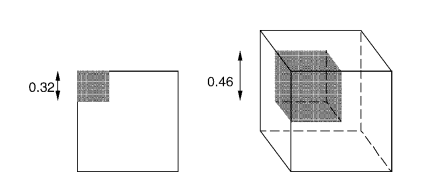
\includegraphics[scale=0.6]{imagenes/radio_alta_dimensionalidad}
		\caption{Para 2 dimensiones necesitamos menor lado que para 3 dimensiones. \cite[p.~64]{cherkassky_learning_2007}}
	\end{figure}
	\item Casi todo punto está más cerca de un borde que de otro punto. Pensemos en un conjunto de datos con $n$ puntos distribuidos de forma uniforme en una bola $d$-dimensional de radio unidad. Para este conjunto de datos, según \cite{hastie_t._elements_nodate}, la distancia media entre el centro de la distribución y los puntos más cercanos a dicho centro se mide bajo la fórmula:
	
	$$D(d,n) = (1-\frac{1}{2}^{1/n})^{1/d}$$
	
	Si en esta fórmula tomamos por ejemplo $n=200$ y $d=10$ el resultado es $D(10,200) \approx 0.57$. Esto significa que los puntos más cercanos al centro de la distribución están más cerca de los bordes que del centro.
	\item Casi todo punto es una anomalía sobre su propia proyección. Si pensamos de nuevo en la idea de los vértices y aristas en espacio de alta dimensionalidad y pensamos en que, según el punto anterior, cada vez que aumenta la dimensionalidad los puntos están más cerca de los bordes entonces no es extraño pensar que los puntos a medida que aumenta la dimensionalidad están más distantes del resto de puntos. Esto intuitivamente (ya que aún no hemos visto la definición formal de anomalía) nos guía a pensar que vistos los puntos en sus propios entornos éstos serán anomalías comparados con el resto.
	
	\begin{figure}[H]
		\centering
		\label{espacio_alta_dimension}
		
\includegraphics[scale=0.6]{imagenes/espacio_alta_dimension}
		\caption{Forma conceptual de un espacio de alta dimensionalidad.\cite[p.~64]{cherkassky_learning_2007}}
	\end{figure}

	Conceptualmente podemos imaginarlo con esta forma de picos, con lo que si tenemos los datos apiñados en dichos picos o extremos el resto de datos que estén en picos diferentes distan tanto del que estamos considerando que no podemos afirmar que tengan ninguna relación entre sí.
\end{enumerate}

Estos puntos hemos de recordar que van referidos al conjunto de datos y no a las funciones que estamos considerando para representar la salida del sistema. Si estamos considerando la complejidad de las funciones la dimensionalidad no es una buena medida. Sabemos de la existencia de teoremas de aproximación de funciones como por ejemplo el Teorema de Superposición de Kolmogorov-Arnold.

\begin{teorema}[Teorema de Superposición de Kolmogorov-Arnold]
	Sea $f$ una función continua de varias variables $f:X_1 \times ... \times X_n \rightarrow \mathbb{R}$, entonces existen funciones $\Phi_q : \mathbb{R}\rightarrow \mathbb{R}$ y $\phi_{q,p} : X_p \rightarrow [0,1]$ tales que $f$ se puede expresar como:
	
	$$f(x) = f(x_1, ..., x_n) = \sum_{q=0}^{2n}\Phi_q ( \sum_{p=1}^{n}\phi_{q,p}(x_p))$$
\end{teorema}

Este Teorema argumenta perfectamente que la complejidad que le damos a los datos por tener una alta dimensionalidad no es transferible a las funciones pues podemos expresar funciones de varias variables como combinación de funciones de una sola variables. En otras palabras no podemos argumentar que la complejidad de funciones univariantes sea mayor o menor que la de funciones multivariantes.

\subsection{Aproximación de funciones}

Como ya hemos dicho en la introducción queremos aproximar una función salida del sistema dentro de una familia de funciones. Este campo no es nuevo, tenemos como herramientas una serie de Teoremas relacionados con la aproximación de funciones como el Teorema de Kolmogorov enunciado anteriormente o el Teorema de aproximación de Weierstrass.

La versión más simple del Teorema de Weierstrass es la de funciones reales definidas en intervalos cerrados, veamos un repaso de estos Teoremas para hacer un esquema de la aproximación de funciones.

\begin{teorema}[Teorema de aproximación de Weierstrass]
	Supongamos que $f:[a,b] \rightarrow \mathbb{R}$ es una función continua. Entonces $\forall \epsilon >0$, $\exists p$ un polinomio tal que $\forall x\in [a,b]$ tenemos que $|f(x)-p(x)|<\epsilon$.
\end{teorema}

En otras palabras, podemos aproximar las funciones continuas reales definidas en un intervalo cerrado con el error que queramos en un punto mediante polinomios. Además tenemos versiones más generales aún como el Teorema de Stone-Weierstrass para funciones reales, para espacios localmente compactos y para el espacio de los complejos.

Estas aproximaciones son más sencillas en términos de la complejidad de la clase de funciones, pero tenemos aproximaciones muy famosas, como por ejemplo la serie de Fourier.

\begin{definicion}[Serie de Fourier]
	Si tenemos una función $f:\mathbb{R} \rightarrow \mathbb{R}$ integrable en el intervalo $[t_0 - \frac{T}{2}, t_0 + \frac{T}{2}]$ entonces se puede obtener el desarrollo en serie de Fourier de $f$ en dicho intervalo. Si $f$ es periódica en toda la recta real la aproximación será válida en todos los valores en los que esté definida.
	
	$$f(t) \approx \frac{a_0}{2} + \sum_{n=1}^{\infty}[a_n \cos (\frac{2n\pi}{T}t) + b_n\sin (\frac{2n\pi}{T}t)]$$
	
	Donde $a_0, a_n$ y $b_n$ son los coeficientes de la serie de Fourier que tienen la forma:
	
	$$a_0 = \frac{2}{T}\int_{-\frac{T}{2}}^{\frac{T}{2}}f(t)dt$$
	
	$$a_n = \frac{2}{T}\int_{-\frac{T}{2}}^{\frac{T}{2}}f(t) cos(\frac{2n\pi}{T}t)dt$$
	
	$$b_n = \frac{2}{T}\int_{-\frac{T}{2}}^{\frac{T}{2}}f(t) \sin (\frac{2n\pi}{T}t)dt$$
\end{definicion}

Como podemos ver hemos introducido dos conocidas formas de aproximar funciones, una con funciones polinómicas y otra con funciones trigonométricas. Vamos a dividir en dos los tipos de  aproximación que podemos tener para el problema de aprendizaje.

\begin{enumerate}
	\item Aproximaciones universales: son aquellas en las que se establece que cualquier función continua puede ser aproximada por otra función de otra clase con el error que queramos. En este grupo podríamos meter a los dos teoremas que hemos dado previamente. Dentro de este grupo podemos tener diferentes tipos de aproximaciones en función de la familia de funciones que escojamos como aproximaciones. Por ejemplo en los dos teoremas previos hemos cogido las clases de funciones polinómicas y trigonométricas pero podríamos haber tomado otras clases diferentes.
	\item Aproximaciones inexactas: son aquellas en las que no podemos tener una aproximación como las que hemos dado en los teoremas previos, si no que proveen de una aproximación de peor calidad.
\end{enumerate}

\subsection{Penalización o control de la complejidad}

Ya hemos discutido brevemente en la sección de principios inductivos la complejidad y cómo penalizarla. Vamos a ver qué elementos queremos controlar con la penalización:

\begin{enumerate}
	\item La clase de funciones con la que vamos a hacer la aproximación. Tenemos que decidir si escoger una clase tan amplia que nos aseguremos que abarque la solución seguro pero penalicemos la complejidad de la elección o queremos una clase de funciones más ajustada.
	\item Tipo de funcional de penalización. Tenemos que escoger entre los distintos tipos de penalización que queremos. Esto se reduce a escoger entre dos tipos de penalización: paramétrica y no paramétrica. La primera de ellas se basa en estudiar la suavidad del ajuste junto con el número de parámetros que requiere la aproximación mientras que la segunda intenta estudiar lo mismo, es decir la suavidad del ajuste, sin medir los parámetros de la clase de funciones. En este punto se puede incorporar el conocimiento a priori del problema.
	\item Método con el que queremos minimizar la penalización. Este apartado está relacionado con los métodos que tenemos de aprender de los datos y el objetivo será intentar hallar una forma eficiente de minimizar tanto el error de la aproximación como la propia penalización.
	\item Control de la complejidad. Como hemos dicho antes el control de la complejidad no es algo sencillo y habrá que escoger la mejor manera de medir dicha complejidad. En secciones posteriores veremos medidas de complejidad como la dimensión de Vapnik-Chervonenkis.
\end{enumerate}

Veamos brevemente la distinción que hemos hecho entre la penalización paramétrica y no paramétrica.

\subsubsection{Penalización paramétrica}

Supongamos que tenemos un conjunto de funciones $f(x,\omega)$ con $\omega \in \Omega$ donde $\Omega$ es el conjunto de parámetros de la forma $\omega = (\omega_0 , ... , \omega_m)$. Como la aproximación viene definida por el parámetros $\omega$ entonces podemos definir también la penalización asociada a dicha selección de parámetros.

Vamos a ver los ejemplos de las penalizaciones más empleadas de este tipo.

\begin{itemize}
	\item Ridge: $\phi_r (\omega_m) = \sum_{i=0}^{m}\omega_i^2$
	\item Selección de subconjunto: $\phi_s (\omega_m) = \sum_{i=0}^{m}\chi (\omega_i \neq 0)$
	\item Bridge: $\phi_p (\omega_m) = \sum_{i=0}^{m}|\omega_i|^p$
	\item Decaimiento de peso: $\phi_q (\omega_m) = \sum_{i=0}^{m}\frac{(\omega_i / q)^2}{1+(\omega_i / q)^2}$ 
\end{itemize}

\subsubsection{Penalización no paramétrica}

En primer lugar vamos a definir la transformada de Fourier de una función para poder definir el funcional de penalización. 

\begin{definicion}[Transformada de Fourier]
	Sea $f$ una función integrable Lebesgue, $f\in L(\mathbb{R})$. Se define la transformada de Fourier de $f$ como la función:
	
	$$\mathcal{F}\{f\} : \xi \rightarrow \hat{f}(\xi) := \int_{-\infty}^{\infty}f(x)e^{-2\pi i\xi x}dx$$
\end{definicion}

Recordemos brevemente las propiedades de la transformada de Fourier.

\begin{itemize}
	\item La transformada de Fourier es un operador lineal: $\mathcal{F}\{a\cdot f + b\cdot g\} = a\mathcal{F}\{f\} + b\cdot \mathcal{F}\{g\}$
	\item $\mathcal{F}\{f(at)\}(\xi) = \frac{1}{|a|}\cdot \mathcal{F}\{f\}(\frac{\xi}{a})$
	\item $\mathcal{F}\{f(t-a)\}(\xi) = e^{-\pi i\xi a}\cdot \mathcal{F}\{f\}(\xi)$
	\item $\mathcal{F}\{f\}(\xi -a) = \mathcal{F}\{e^{\pi iat}f(t)\}(\xi)$
	\item $\mathcal{F}\{f'\}(\xi) = 2\pi i\xi \mathcal{F}\{f\}(\xi)$
	\item $\mathcal{F}\{f\}'(\xi) = \mathcal{F}\{(-it)\cdot f(t)\}(\xi)$
\end{itemize}

Habiendo recordado esto podemos definir el funcional de penalización no paramétrica. Este funcional mide la suavidad del ajuste de la función gracias a que se puede medir, mediante la transformada de Fourier, la ondulación de la función. Por tanto el funcional no paramétrico que se propone es:

$$\phi [f] = \int_{\mathbb{R}^d}\frac{|\hat{f}(s)|^2}{\hat{G}(s)}ds$$

Donde $\hat{f}$ indica la transformada de Fourier de la función $f$ y $\frac{1}{\hat{G}}$ es la transformada de Fourier de una función de filtro de paso alto. Es en esta proposición de filtro donde se añade el conocimiento a priori del problema. Por ejemplo pudiera ser interesante en alguna aplicación práctica tener un funcional invariante frente a rotaciones de funciones.

\subsection{Equilibrio entre el sesgo y la varianza}

Este enfoque es muy utilizado en el estudio del error, dividiéndolo en sesgo y varianza para hacer un mejor estudio del mismo y poder enfrentar ambos con varios métodos. Este estudio del caso clásico no es válido (o al menos no del todo) para problemas no supervisados como es nuestro caso. Vamos a hacer una adaptación de esta teoría para que pueda encajar en nuestro caso de estudio.

Tenemos que tener en cuenta que no conocemos la salida real del sistema en el caso de detección de anomalías, es decir, no sabemos estimar con certeza el sesgo y la varianza y por tanto el error que cometemos. En primer lugar vamos a ver una pequeña adaptación de la notación al caso de detección de anomalías para poder hacer un estudio enfocado.

Vamos a notar por $X_1 , ... , X_n$ los datos de test y $\mathcal{D}$ como conjunto de datos de entrenamiento. Además vamos a considerar que existe una función $f$ que nos da la etiqueta real de un dato, esto es, si es o no una anomalía. Por tanto podemos decir que la auténtica etiqueda de un dato es $y_i = f(X_i)$. Además nosotros estaremos usando un modelo ya escogido por nosotros para predecir la etiqueta de un dato de test, esto es $g(X_i, \mathcal{D})\approx y_i+\beta$ donde $\beta$ es un cierto error.

Una vez conocida esta notación podemos definir el error medio al cuadrado como:

$$MSE = \frac{1}{n}\sum_{i=1}^{n}\{y_i - g(X_i, \mathcal{D})\}^2$$

Y podemos definir también el valor esperado del error medio al cuadrado como:

$$E[MSE] = \frac{1}{n} \sum_{i=1}^{n}E[\{y_i - g(X_i, \mathcal{D}\}^2]$$

Una vez definido el $MSE$ esperado podemos desarrollar un poco el cálculo para poder obtener el error y la varianza que esperamos.

En primer lugar podemos escribirlo como:

$$E[MSE] = \frac{1}{n}\sum_{i=1}^{n}E[\{ (y_i-f(X_i)) + (f(X_i) - g(X_i,\mathcal{D})) \}^2]$$

Aquí solo hemos restado y sumado $f(X_i)$, ahora si recordamos que $y_i = f(X_i)$ entonces podemos igualar el primero de los paréntesis a $0$ y por tanto nos queda:

$$E[MSE] = \frac{1}{n}\sum_{i=1}^{n}E[\{ f(X_i) - g(X_i, \mathcal{D}) \}^2]$$

Si seguimos descomponiendo podemos sumar y restar $E[g(X_i, \mathcal{D})]$ con lo que nos quedaría:

$$E[MSE] = \frac{1}{n}\sum_{i=1}^{n}E[\{ f(X_i) - E[g(X_i, \mathcal{D})] \}^2]$$

$$ + \frac{2}{n}\sum_{i=1}^{n}\{ f(X_i) - E[g(X_i, \mathcal{D})] \}\cdot \{ E[g(X_i, \mathcal{D})] - E[g(X_i, \mathcal{D})] \}$$

$$ + \frac{1}{n}E[\{ E[g(X_i, \mathcal{D}) - g(X_i, \mathcal{D})] \}^2]$$

Como es claro, el segundo término da cero por lo que nos queda al final:

$$E[MSE] = \frac{1}{n} \sum_{i=1}^{n}E[\{ f(X_i) - E[g(X_i, \mathcal{D})] \}^2] + \frac{1}{n}\sum_{i=1}^{n}E[\{ E[g(X_i, \mathcal{D})] - g(X_i, \mathcal{D}) \}^2]$$

$$=\frac{1}{n}\sum_{i=1}^{n}\{ f(X_i) - E[g(X_i, \mathcal{D})] \}^2 + \frac{1}{n}\sum_{i=1}^{n}E[\{ E[g(X_i, \mathcal{D})] - g(X_i, \mathcal{D}) \}^2]$$

Si reconocemos cada uno de los términos, en primer lugar el primero de ellos es el sesgo al cuadrado y el segundo la varianza, por lo que finalmente lo que hemos obtenido es:

$$E[MSE] = sesgo^2 + varianza$$

El dilema que se nos plantea es el siguiente: si tomamos modelos con un bajo sesgo en la estimación de los parámetros entonces tendremos una alta varianza y viceversa. Esto significa que no podemos con el conocimiento del que disponemos disminuir tanto el sesgo como la varianza a la vez. Es esta propiedad la que se conoce como la compensación entre sesgo y varianza.

\section{Teoría estadística del aprendizaje}

En esta sección vamos a hacer un repaso por la teoría del aprendizaje, en concreto la teoría desarrollada por Vapnik-Chervonenkis. Esta teoría se basa o tiene como pilares cuatro puntos:

\begin{enumerate}
	\item Condiciones para la consistencia del principio ERM o minimización del error empírico.
	\item Cotas en la capacidad de generalización de las máquinas de aprendizaje.
	\item Principios de inferencia sobre muestras finitas.
	\item Métodos constructivos para implementar los principios inductivos ya expuestos.
\end{enumerate}

Durante el desarrollo de esta sección haremos un repaso de estos cuatro puntos para dar el broche final a esta sección y poder realizar la primera de las definiciones de anomalía.

\subsection{Condiciones para la convergencia y consistencia del ERM}

En el problema de aprendizaje disponemos de una muestra en la que tenemos los propios datos de entrada y la salida del sistema. Denotemos a estos elementos por $z=(x,y)$ donde $x$ son los datos de entrada e $y$ la salida del sistema. Por tanto la muestra que se nos da es un conjunto $Z_n = \{ z_1 , ... , z_n \}$. Estos datos están generados como ya sabemos mediante una función de densidad desconocida $p(z)$. Sobre este esquema tenemos una serie de funciones de pérdida y un funcional de pérdida. El objetivo es encontrar dicha función de pérdida $Q(z,\omega )$ que minimice dicho funcional:

$$R(\omega) = \int Q(z,\omega) p(z)dz$$

Por tanto si tenemos la función de pérdida podemos definir el error empírico como:

$$R_{emp}(\omega) = \sum_{i=1}^{n}Q(z_i, \omega)$$

Donde $\omega$ son los parámetros escogidos para el modelo.

Para poder estudiar la consistencia del ERM primero debemos definir formalmente dicha propiedad. Denotamos por $R_{emp}(\omega_n^*)$ el valor del error empírico con la función de pérdida $Q(z,\omega_n^*)$ que minimiza el error empírico para el conjunto de entrenamiento $Z_n$. Denotemos además por $R(\omega_n^*)$ el verdadero valor (desconocido) del error para la función de pérdida. Como se puede ver estos valores dependen del tamaño del conjunto de entrenamiento $n$, podemos por tanto estudiar cómo se comportan estos errores cuando aumentamos el tamaño del conjunto de entrenamiento. Es aquí donde entra la definición de consistencia del ERM. Decimos que es consistente si la sucesión de errores reales y empíricos convergen en probabilidad al mismo límite $R(\omega_0) = \min_{\omega} R(\omega)$. Es decir:

$$R(\omega_n^*) \rightarrow R(\omega_0) \ cuando \ n\rightarrow \infty$$
$$R_{emp}(\omega_n^*) \rightarrow R(\omega_0) \ cuando \ n\rightarrow \infty$$

Para poder asegurar esta propiedad sobre el ERM tenemos el conocido como Teorema Clave de la Teoría del Aprendizaje de Vapnik y Chervonenkis.

\begin{teorema}[Teorema Clave de la Teoría del Aprendizaje]
	Para funciones de pérdida acotadas el principio inductivo de minimización del error empírico es consistente sí y sólo si el error empírico converge uniformemente al valor real del error en el siguiente sentido:
	
	$$\lim\limits_{n\rightarrow \infty} P[\sup_{\omega}|R(\omega) - R_{emp}(\omega)|>\epsilon] = 0 \ , \ \forall \epsilon >0$$
\end{teorema}

Cabe recalcar que estas condiciones de consistencia dependen de las propiedades de la clase de funciones elegida. No podemos pretender escoger como clase de aproximación una muy general y seguir manteniendo las condiciones de consistencia del ERM. Aún así el teorema nos está dando condiciones generales para la consistencia del ERM pero son abstractas y no fácilmente aplicables en la práctica. Para ello vamos a estudiar las condiciones de convergencia de ERM que sí serán aplicables en la implementación de algoritmos.

Vamos ahora a particularizar el estudio en el caso de clasificación binaria por ser la materia de estudio que nos ocupa, pues al final tendremos que clasificar instancias en anómalas o no anómalas. Ahora las funciones de pérdida $Q(z,\omega)$ son funciones de pérdida indicadoras. Vamos a notar por $N(Z_n)$ el número de dicotomías que se pueden tener con la clase de funciones elegidas. Esto es el número de formas de clasificar los datos en las dos clases existentes.

Una vez actualizada nuestra notación podemos definir la entropía aleatoria como $H(Z_n) = \ln N(Z_n)$. Esta cantidad es una variable aleatoria dependiente de los valores de entenamiento $Z_n$, podemos definir ahora la entropía de Vapnik-Chervonenkis como el valor medio o esperado de la entropía aleatoria:

$$H(n) = E[\ln N(Z_n)]$$

Esta medida es una cuantificación de la diversidad del conjunto de funciones indicadoras que nos pueden separar los datos en ambas clases.

Por último vamos a definir la función de crecimiento que nos va a permitir hacer cotas y llegar a la condición necesaria y suficiente para la convergencia del ERM. Definimos la función de crecimiento como:

$$G(n) = \ln \max_{Z_n} N(Z_n)$$

Donde aquí estamos notando el máximo número de dicotomías sobre todas las posibles muestras existentes de tamaño $n$. Es más, como el máximo número de formas de dividir un conjunto de tamaño $n$ en dos clases es $2^n$ entonces podemos afirmar que $G(n)\leq n\ln (2)$.

Por último y para completar la cadena de desigualdades que buscamos vamos a definir la entropía reforzada de Vapnik-Chervonenkis:

$$H_{ann}(n) = \ln (E[N(Z_n)])$$

Haciendo uso de la conocida desigualdad de Jensen

$$\sum_{i=1}^{n}a_i \ln (x_i) \leq \ln (\sum_{i=1}^{n}a_i x_i)$$

podemos ver claramente que $H(n)\leq H_{ann}(n)$. Por tanto obtenemos la cadena de desigualdades:

$$H(n)\leq H_{ann}(n) \leq G(n) \leq n\ln (2)$$

La condición necesaria y suficiente de Vapnik-Chervonenkis para la convergencia del ERM que hallaron fue que:

$$\lim\limits_{n\rightarrow \infty} \frac{H(n)}{n} = 0$$

Pero esta condición no asegura una convergencia rápida asintóticamente al error real. Se dice que el ratio de convergencia es rápido asintóticamente en la Teoría de Vapkin-Chervonenkis si:

$$\forall n>n_0 \ P(R(\omega) - R(\omega^*)<\epsilon) = e^{-cn\epsilon^2} \ con \ c>0$$

Para poder cumplir esta condición se dio la condición suficiente para la convergencia rápida:

$$\lim\limits_{n\rightarrow \infty} \frac{H_{ann}(n)}{n} = 0$$

Estas condiciones son dependientes de la distribución de los datos $Z_n$ como es claro al depender de la esperanza de una variable aleatoria dependiente de $Z_n$. Es por tanto que esta condición no es del todo general. Para solventar esto se tiene la consistencia y convergencia del ERM con la condición necesaria y suficiente de que:

$$\lim\limits_{n\rightarrow \infty}\frac{G(n)}{n}$$

Por tanto este estudio nos ha dado las condiciones de convergencia y consistencia del ERM.

\chapter{Concepto de anomalía}
\label{chapter:anomalia}
%
\chapter{Concepto de anomalía}
\label{chapter:anomalia}

\section{Contextualización}

Ya hemos discutido previamente una idea intuitiva del concepto de anomalía. Un dato decimos que es anómalo cuando se distancia del resto de los datos lo suficiente como para no tener características comunes con ellos.

Este hecho puede ser por distintos motivos. Puede que la anomalía venga del hecho de que se está produciendo un evento en nuestros experimentos que no sea nada frecuente. Por ejemplo podemos estar midiendo datos meteorológicos y que en un momento dado se den una serie de fenómenos que no sea frecuente ver juntos, o incluso que no se hayan visto nunca ocurrir simultáneamente. Otra forma de tener una anomalía en nuestro conjunto de datos pudiera ser errores de medición. Por ejemplo si seguimos con este símil de los datos meteorológicos imaginemos que nuestra estación dispone de un termómetro. Este sensor se ha roto y empieza a marcar datos superiores a 100 $C^\circ$, claramente son datos muy desviados de las temperaturas normales con lo que no tendrían relación con el resto y presentaría una desviación muy importante con respecto al resto de los datos.

\section{Criterios}

Esta idea intuitiva que estamos dando de anomalía no refleja todos los posibles escenarios. Los ejemplos que estamos dando suponen una desviación muy grande de los datos normales, tanto que no se pueden comparar con el resto porque difieren mucho numéricamente. Vamos a plantear un escenario para dar una mejor forma al concepto de anomalía. Pensemos en una serie de datos muy agrupados en dos clústeres por ejemplo:

\begin{figure}[H]
	\centering
	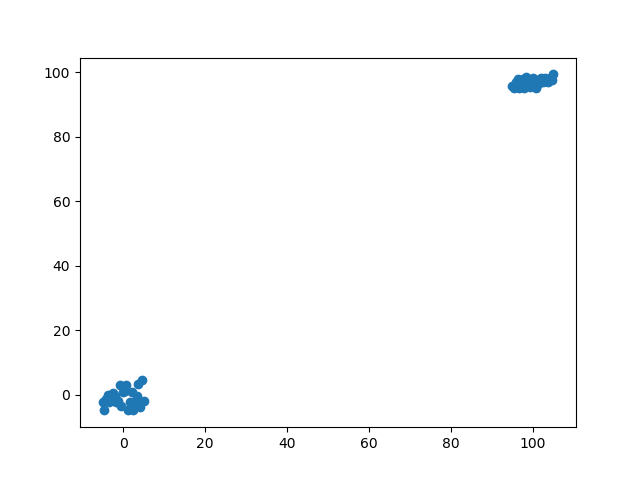
\includegraphics[scale=0.5]{imagenes/clusters}
	\label{clusters}
	\caption{Clústeres alejados}
\end{figure}

Como podemos comprobar que tenemos dos clústeres no sólo alejados entre sí, si no con los elementos muy concentrados para poner un caso extremo. Ahora no vamos a proponer un valor que se aleje de los dos clústeres, si no uno que esté a medio camino entre los dos:

\begin{figure}[H]
	\centering
	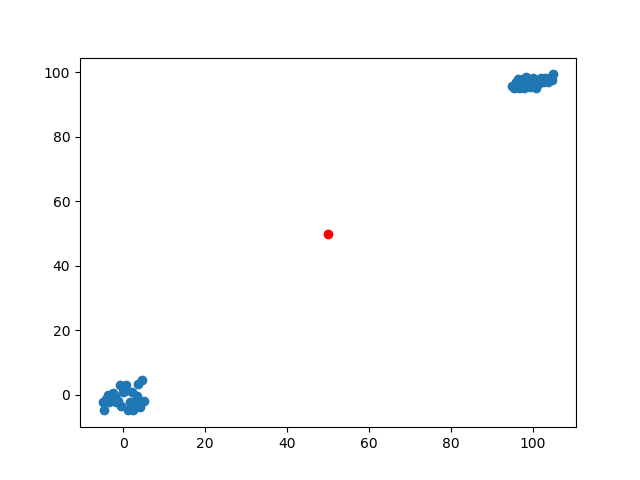
\includegraphics[scale=0.5]{imagenes/outlier_cluster}
	\label{outlier_clusters}
	\caption{Clústeres alejados con una anomalía en rojo}
\end{figure}

Si los datos del clúster de abajo a la izquierda fueran datos de temperatura con valores entorno a 0 y los de arriba a la derecha fueran de datos de temperatura entorno a 100 grados nuestro datos anómalo tendría una temperatura de unos 50 grados. Esta temperatura no se aleja radicalmente de los valores normales, es decir, no son -1000 grados ni 1000 grados. Aún así estamos describiendo una situación anómala.

No podemos dar una definición formal o que podamos decir que abarca todos los casos para definir lo que es una anomalía, aún así vamos a intentar dar dos puntos de vista: uno basado en distancias y otro en probabilidades.

El criterio más usado en la definición o detección de anomalías es el llamado ``Tukey's Fences''. Para introducirlo vamos a ver su definición en una única dimensión para luego extender el concepto. Pensemos en un conjunto de datos 1-D. Sobre sus valores podemos calcular los cuartiles $Q_1 , Q_2 $ y $Q_3$. Un valor anómalo es aquel que no cae dentro del intervalo $[Q_1 - k(Q_3 - Q_1), Q_3 + k(Q_3 - Q_1)]$ donde $k$ es una constante. El valor propuesto para $k$ por Tukey fue de $k=1.5$ aunque algunos autores más restrictivos proponen $k=3$.

Este criterio puede ser extendido al caso de mayor dimensionalidad si realizamos este mismo test sobre todos los valores de todas las características y comprobar si alguno o todos se salen del rango en función de cómo de restrictivo queremos que sea el criterio.

Esta extensión es muy vaga, por lo que se propone un criterio un poco más fijado. Imaginemos los datos agrupados por clústeres, entonces podemos fijar un centroide de dicho clúster. Sobre cada clúster podemos medir cuál es la mayor distancia dentro del clúster de los datos al centroide. Podemos extender el criterio de Tukey diciendo que un dato anómalo es aquel que se distancia más de $1.5$ veces de la mayor distancia dentro del clúster al centroide.

Esta generalización ya si abarca el ejemplo que hemos propuesto. Al estar muy apiñados los datos entorno al centroide la mayor distancia dentro del clúster es muy pequeña, de hecho en el ejemplo construido es menor que 5. Por tanto el dato $(50,50)$ está alejado más de $1.5 \cdot 5 = 7.5$ unidades del centroide y por tanto lo podemos considerar una anomalía.

\section{Qué hacer con las anomalías}

Estamos estudiando cómo podemos detectar anomalías pero una vez que las hayamos detectado en nuestros conjuntos de datos en un problema real, ¿qué debemos hacer con ellas? Este problema es algo muy general, puede que estemos seguros en nuestro caso de que las anomalías se han debido a un problema de medición porque nuestros instrumentos estaban rotos y por tanto deberíamos descartarlos. Puede que sean datos reales pero estén tan separados del resto que debamos estudiarlos de forma separada. Vamos a dar unas cuantas alternativas a lo que podemos hacer una vez que hemos detectados las anomalías dentro de nuestro conjunto de datos:

\begin{itemize}
	\item Dejarlos: puede que nuestro conjunto de datos tenga un número de datos muy elevado y por tanto aparezcan en él anomalías. Estas anomalías no deben ser eliminadas, es más debemos escoger modelos que aprendan o utilicen los datos teniendo en cuenta estas anomalías y siendo robustos ante su aparición.
	\item Exclusión: una opción es eliminar directamente las anomalías. Esto en general no está justificado y de hecho no se recomienda pues perdemos riqueza del conjunto de datos al eliminar instancias del mismo. Aún así, si decidimos eliminar los datos tenemos dos formas de hacerlo. Podemos eliminarlos directamente y prescindir de esos datos o podemos sustituirlos por datos cercanos que no sean anómalos.
	\item Estudiarlos por separado: puede que tengamos un número suficientemente elevado de las mismas y que enseñen algunos patrones o tengan explicación en nuestro ejemplo del mundo real. En este caso quizás deberíamos considerarlas y estudiarlas a parte para darles un sentido y emplear el conocimiento que les subyace.
\end{itemize}
%
\chapter{Introducción de Estadística Multivariante}
\label{chapter:estadistica_multivariante}

Vamos a dar otra definición de anomalía que no coincide con la que hemos visto basada en distancias, pero antes de dar esa definición debemos hacer un breve repaso de estadística multivariante y probabilidad para poder comprender y enmarcar dicha definición.

\section{Introducción}

En primer lugar vamos a describir conceptos básicos sobre los que poder construir los conceptos que necesitamos para la definición de anomalía basada en probabilidades.

En primer lugar vamos a definir el concepto de variable aleatoria.

\begin{definicion}
	Una variable aleatoria es una función $X:\Omega \rightarrow E$ que parte de un espacio de probabilidad $(\Omega , \mathcal{F}, \mathcal{P})$ y llega a un espacio medible $(E, \mathcal{B})$, donde $X$ además es una función medible.
\end{definicion}

Normalmente ya sabemos que $E\subseteq \mathbb{R}$ y además cabe recordar que $\mathcal{F}$ es una $\sigma$-álgebra. Además cabe recordar la definición de función medible:

\begin{definicion}
	Decimos que una función $X: (\Omega , \mathcal{F}, \mathcal{P}) \rightarrow (E, \mathcal{B})$ es medible si $X^{-1}(B)\subset \mathcal{F}$, $\forall B \in \mathcal{B}$.
\end{definicion}

Esta definición puede extenderse al caso vectorial, introduciendo con esto la noción de vector aleatorio:

\begin{definicion}
	Un vector aleatorio $\underline{X} = (X_1 , ... , X_p)$ es una aplicación medible $\underline{X}: (\Omega , \mathcal{F}, \mathcal{P})\rightarrow (E, \mathcal{B}^p)$ donde $E\subseteq \mathbb{R}^p$.
\end{definicion}

Se puede demostrar además la caracterización:

\begin{proposicion}
	Un vector $\underline{X} = (X_1, ..., X_p)$ es un vector aleatorio si y sólo si $X_i : (\Omega , \mathcal{F}, \mathcal{P}) \rightarrow (\mathbb{R}, \mathcal{B})$ es una función medible.
\end{proposicion}

Con este vector aleatorio podemos estudiar o definir la distribución de probabilidad del mismo sobre $( \mathbb{R}^p , \mathcal{B}^p )$ $P_{\underline{X}}$ como:

$$P_{\underline{X}} [B]:= P[\underline{X}^{-1}(B)] \ \forall B\in \mathcal{B}$$

con lo que el espacio $(\mathbb{R}^p , \mathcal{B}^p , P_{\underline{X}})$ es un espacio de probabilidad o probabilístico.

Sobre los conocimientos de la definición de la función de distribución univariante podemos hacer una definición análoga para el caso multivariante.

\begin{definicion}
	Se define la función de distribución asociada a la probabilidad inducida como:
	
	$$F_{\underline{X}} (\underline{x}) = P_{\underline{X}} [X_1 \leq x_1 , ... , X_p \leq x_p] \ , \ \forall \underline{x} = (x_1 , ... , x_p) \in \mathbb{R}^p$$
\end{definicion}

De igual forma podemos caracterizar la función de densidad como aquella $f_{\underline{X}}$ que, de existir, cumple que:

$$F_{\underline{X}} (\underline{x}) = \int_{- \infty}^{x_1} \int_{-\infty}^{x_2} ... \int_{-\infty}^{x_p} f_{\underline{X}}(u_1 , ... , u_p) du_1 ... du_p$$

Otra forma de determinar de forma única la distribución de un vector aleatorio es mediante la función característica, lo que nos va a dar además una caracterización de la independencia que introduciremos en siguiente lugar.

\begin{definicion}
	Dado un vector aleatorio $X = (X_1 , ... , X_p)$ se define la función característica como $\Phi_{\underline{X}} (\underline{t}) = E[e^{i\underline{t}X}]$ con $\underline{t} = (t_1 , ... , t_p)\in \mathbb{R}^p$ donde la función $E[\cdot]$ denota la esperanza, por lo que:
	$$\Phi_{\underline{X}} (\underline{t}) = \int_{\mathbb{R}^p} e^{i\underline{t} \underline{X}} P_{\underline{X}}(d\underline{x})$$
\end{definicion}

Con esto ya podemos introducir el concepto de independencia en varias variables. 

\subsection{Independencia}

\begin{definicion}
	Dados dos vectores aleatorios $\underline{X} = (X_1 , ... , X_p)$, $\underline{Y} = (Y_1 , ... , Y_p)$ se dice que son independientes si:
	$$F_{\underline{X}, \underline{Y}}(\underline{x}, \underline{y}) = F_{\underline{X}}(\underline{x}) \cdot F_{\underline{Y}}(\underline{y})$$
\end{definicion}

Podemos también definir la independencia entre las variables de un vector aleatorio como:

\begin{definicion}
	$X = (X_1 , ... , X_p)$ se dice que está compuesto de variables independientes si $\forall B = B_1 \times ... \times B_p$ con $B_i \in \mathcal{B}$ se tiene que:
	
	$$P_{\underline{X}}(B) = P_{X_1}[B_1] \cdot ... \cdot P_{X_p}[B_p]$$
\end{definicion}

En cuanto a la independencia de sucesos podemos dar dos definiciones de independencia:

\begin{definicion}
	Decimos que los eventos $B = (B_1 , ... , B_p)$ son independientes dos a dos si para todos $m\neq k$ se tiene que $P(B_m \bigcap B_k) = P(B_m)P(B_k)$
\end{definicion}

\begin{definicion}
	Se dice que los eventos $B = (B_1 , ... , B_p)$ son independientes mutuamente si para todo $k\leq p$ se tiene que $P(\bigcap_{i=1}^{k}B_i) = \prod_{i=1}^{k}(B_i)$
\end{definicion}

En cuanto a la definición de independencia entre las variables aleatorias que definen un vector aleatorio podemos dar dos caracterizaciones basadas en la función característica.

\begin{proposicion}
	Si las componentes del vector aleatorio $X = (X_1 , ... , X_p)$ son independientes entonces:
	
	$$\Phi_{\underline{X}}(\underline{t}) = E[e^{i\underline{t}\underline{X}}] = \prod_{j=1}^{p}E[e^{it_j X_j}]$$
\end{proposicion}

\begin{proposicion}
	Si las componentes del vector aleatorio $X = (X_1 , ... , X_p)$ son independientes entonces la función característica de la variable $Y = \sum_{j=1}^{p}X_j$ es:
	
	$$\Phi_Y (t) = E[e^{itY}] = E[e^{it \sum_{j=1}^{p}X_j}] = \prod_{j=1}^{p}\Phi_{X_j} (t)$$
\end{proposicion}

\subsection{Probabilidad y esperanza condicionada}

En esta sección vamos a describir la probabilidad y esperanza condicionada de una variable aleatoria y no de un vector aleatorio. Este hecho es sencillo de deducir, pues como hemos introducido previamente la distribución de probabilidad de un vector aleatorio viene determinada por una distribución de probabilidad de una variable aleatoria. Por tanto el estudio de la probabilidad y esperanza condicionada en el caso univariante se hace válido para el caso multivariante. 

En primer lugar debemos introducir el concepto de probabilidad condicionada tal y cómo la conocemos hasta ahora de Bayes. Partimos de un espacio de probabilidad $(\Omega , \mathcal{A}, \mathcal{P})$.

\begin{definicion}
	Definimos la probabilidad condicionada a un suceso $B\in \mathcal{A}$ con $P(B)>0$ como:
	
	$$P(\cdot | B) : \mathcal{A} \rightarrow [0,1] , \ \ \ P(A | B) = \frac{P(A\cap B)}{P(B)}$$
\end{definicion}

Esta es una función de probabilidad, por lo que nos lleva a pensar en el espacio de probabilidad que genera, es más podemos pensar en el espacio de probabilidad en el que la probabilidad condicionada no se anula, es decir:

$$\mathcal{A}_B = \{ C = A\cap B, \ A\in \mathcal{A} \}$$

Por tanto solemos considerar como espacio de probabilidad condicionada al espacio $(B, \mathcal{A}_B , P(\cdot | B))$.

Partiendo de este espacio de probabilidad podemos considerar una variable aleatoria $X : (\Omega , \mathcal{A}, \mathcal{P}(\cdot | B)) \rightarrow (\mathbb{R}, \mathcal{B})$. 

\begin{definicion}
	Definimos la esperanza de esta variable aleatoria condicionada a $B$ como:
	$$E[X | B] = \int_{\Omega}XdP(\cdot | B) = \int_{\Omega}XdP(\cdot | B) = \frac{1}{P(B)}\int_{B}XdP = \frac{E[X1_B]}{P(B)}$$
	Donde $1_B$ representa la función indicadora del conjunto $B$.
\end{definicion}

No sólo podemos estudiar la probabilidad y esperanzas condicionadas a un evento, si no que también las podemos estudiar condicionadas a una $\sigma$-álgebra. En este terreno vamos a distinguir dos posibilidades: condicionamiento a una $\sigma$-álgebra generada por una partición numerable de sucesos de probabilidad no nula y condicionamiento a una $\sigma$-álgebra arbitraria.

\begin{definicion}
	Definimos la esperanza condicionada a una $\sigma$-álgebra $\mathcal{A}$ generada por $\{ B_n \}\subset \mathcal{A}$ con $B_i \cap B_j = \phi , \ i\neq j$, $\bigcup_{n=1}^{\infty} B_n = \Omega$ y $P(B_i)>0 , \ \forall i$. Siendo la $\mathcal{U} = \sigma (\{ B_n \})$ la $\sigma$-álgebra generada por $\{ B_n \}$. Con este marco, definimos la esperanza de una variable aleatoria $X: (\Omega , \mathcal{A}, P) \rightarrow (\mathbb{R}, \mathcal{B})$ condicionada a la $\sigma$-álgebra $\mathcal{U}$ como:
	
	$$E[X | \mathcal{U}](\omega) = \sum_{n=1}^{\infty} E[X | B_n]1_{B_n}(\omega)$$
\end{definicion}

\begin{propiedades}
	\begin{enumerate}
		\item $E[X | \mathcal{U}]: (\Omega , \mathcal{U}) \rightarrow (\mathbb{R}, \mathcal{B})$ es $\mathcal{U}$-medible.
		\item $E[E[X | \mathcal{U}]] = \sum_{n=1}^{\infty}E[X | B_n]P(B_n) = \sum_{n=1}^{\infty}E[X1_{B_n}] = E[X]$
	\end{enumerate}
\end{propiedades}

De igual forma podemos definir la probabilidad condicionada a una $\sigma$-álgebra generada por una partición numerable de sucesos no nulos.

\begin{definicion}
	Definimos la probabilidad de un suceso $A\in \mathcal{A}$ condicionada a la $\sigma$-álgebra $\mathcal{U}$ como:
	
	$$P(A | \mathcal{U}) = E[1_A | \mathcal{U}] = \sum_{n=1}^{\infty}E[1_A | B_n]1_{B_n} = \sum_{n=1}^{\infty}P(A | B_n)1_{B_n}$$ casi seguramente.
\end{definicion}

Podemos también dar unas propiedades inmediatas de la probabilidad condicionada tomando como base las de la esperanza.

\begin{propiedades}
	\begin{enumerate}
		\item $P(A | \mathcal{U})$ es $\mathcal{U}$-medible.
		\item $E[P(A | \mathcal{U})] = P(A)$
	\end{enumerate}
\end{propiedades}

Una vez visto esto podemos hacer una definición con una $\sigma$-álgebra arbitraria. Cabe decir que en este caso no vamos a poder dar una definición constructiva y fácil de calcular como sí hemos hecho en el caso particular anterior. Lo que sí vamos a tener con esta definición más general es el mantenimiento de las propiedades que hemos visto en primera instancia tanto de la probabilidad como de la esperanza condicionada. Sobra decir además que esta definición coincide con la anterior en el caso particular de una $\sigma$-álgebra generada por una partición numerable de sucesos no nulos.

\begin{definicion}
	Definimos la esperanza de una variable aleatoria $X$ en el marco dado condicionada a una $\sigma$-álgebra $\mathcal{U}\subset \mathcal{A}$ como la única función $\mathcal{U}$-medible tal que:
	
	$$\forall u \in \mathcal{U} \ \int_{\mathcal{U}}E[X | \mathcal{U}]P_{\mathcal{U}} = \int_{\mathcal{U}}X dP$$ casi seguramente $P_{\mathcal{U}}$. Donde $\forall u\in \mathcal{U}$ $P_{\mathcal{U}}(u) = P(u)$.
\end{definicion}

Igualmente podemos dar una definición de la probabilidad condicionada a una $\sigma$-álgebra arbitraria tomando como base la definición de esperanza condicionada.

\begin{definicion}
	Definimos la probabilidad de $A\in \mathcal{A}$ condicionada a la $\sigma$-álgebra $\mathcal{U}$ como:
	
	$$P(A | \mathcal{U}) = E[1_A | \mathcal{U}]$$ casi seguramente $P_{\mathcal{U}}$.
\end{definicion}

Por último antes de dar unas propiedades que nos den un poco más de conocimiento y herramientas de trabajo vamos a ver el concepto de probabilidad y esperanza condicionada a una variable aleatoria y no a un suceso o una $\sigma$-álgebra como hemos visto previamente.

Partimos igualmente del marco $(\Omega , \mathcal{A} , P)$ con dos variables aleatorias $X,Y$.

\begin{definicion}
	Definimos la $\sigma$-álgebra generada por la variable aleatoria $Y$ como la menor $\sigma$-álgebra que hace medible a la variable aleatoria $Y$ y la notaremos como $\sigma (Y)$.
\end{definicion}

Ahora si podemos definir la esperanza de una variable aleatoria condicionada a otra.

\begin{definicion}
	Definimos la esperanza de la variable aleatoria $X$ condicionada a la variable aleatoria $Y$ como:
	$$E[X | Y] = E[X | \sigma (Y)]$$
\end{definicion}

Como anotación cabe decir que esta esperanza condicionada es una función dependiente de la variable aleatoria $Y$, es decir podemos expresarla como:

$$g(y) = E[X | Y=y]$$

Ahora que tenemos la definición de la esperanza condicionada a una variable aleatoria podemos usar el concepto como hemos hecho anteriormente para definir la probabilidad de un suceso condicionado a una variable aleatoria.

\begin{definicion}
	Para todo $A\in \mathcal{A}$ definimos la probabilidad de $A$ condicionada a la variable aleatoria $Y$ como:
	$$P(A | Y) = E[1_A | \sigma (Y)]$$
	casi seguramente $P_{\sigma (Y)}$
\end{definicion}

Ahora estamos en condiciones de dar una propiedades elementales y de suavizamiento que nos van a dar herramientas con las esperanzas condicionadas. En este punto ya hemos visto que, al haber hecho las definiciones de esperanza y probabilidades usándolas indistintamente las propiedades que vamos a dar para la esperanza se pueden emplear para las probabilidades utilizando sus definiciones que impliquen el uso de esperanzas.

Sobre estas propiedades vamos a realizar algunas de las demostraciones de las propiedades elementales y de las de suavizamiento que vamos a dar para poner de relieve cómo podemos hacer uso de la probabilidad y esperanza condicionada.

\begin{propiedades}[Propiedades elementales]
	Partimos de un espacio de probabilidad $(\Omega , \mathcal{A}, P)$, $\mathcal{U}$ una $\sigma$-álgebra contenida en $\mathcal{A}$ y $X,Y$ variables aleatorias integrables.
	\begin{enumerate}
		\item $E[cte | \mathcal{U}] = cte$ casi seguramente $P_{\mathcal{U}}$
		\item Sean $a, b \in \mathbb{R}$ $E[aX + bY | \mathcal{U}] = aE[X | \mathcal{U}] + bE[Y | \mathcal{U}]$ casi seguramente $P_{\mathcal{U}}$, es decir, la esperanza condicionada cumple la propiedad de linealidad.
		\item $X\geq Y$ casi seguramente $P$ $\Rightarrow E[X | \mathcal{U}] \geq E[Y | \mathcal{U}]$ casi seguramente $P_{\mathcal{U}}$.
		\item $|E[X | \mathcal{U}]| \leq  E[|X| |\mathcal{U}]$
	\end{enumerate}
\end{propiedades}

\begin{demostracion}
	Vamos a demostrar la propiedad 1 para ver como trabajar con las igualdades casi seguras.
	\begin{enumerate}
		\item[1.] Como la igualdad es casi seguramente podemos aplicar integrales en la misma con lo que obtenemos lo siguiente:
		$$\forall u \in \mathcal{U} \ \int_{u} E[cte | \mathcal{U}]dP_{\mathcal{U}} = \int_{u}cte dP = cte P(u) = cte P_{\mathcal{U}}(u) = \int_{u}cte dP_{\mathcal{U}}$$
		Como la igualdad es con integrales, podemos decir por tanto que $E[cte | \mathcal{U}] = cte$ casi seguramente $P_{\mathcal{U}}$.
	\end{enumerate}
\end{demostracion}

\begin{propiedades}[Propiedades de suavizamiento]
	Partimos del marco del espacio probabilístico $(\Omega , \mathcal{A}, P)$ con una $\sigma$-álgebra $\mathcal{U}\subset \mathcal{A}$.
	\begin{enumerate}
		\item Si $X$ es una variable aleatoria integrable y $\mathcal{U}$-medible entonces se tiene que $E[X | \mathcal{U}] = X$ casi seguramente $P_{\mathcal{U}}$
		\item Sean $X, Y$ variables aleatorias con $X$ $\mathcal{U}$-medible, $Y$ integrable y $XY$ integrable, entonces se tiene que $E[XY | \mathcal{U}] = XE[Y | \mathcal{U}]$ casi seguramente $P_{\mathcal{U}}$.
		\item Se dice que $X$ es independiente de $\mathcal{U}$ si $X$ y $1_{\mathcal{U}}$ son independientes. Si $X$ es independiente de $\mathcal{U}$ entonces $E[X | \mathcal{U}] = E[X]$ casi seguramente $P_{\mathcal{U}}$.
		\item Sean $\mathcal{U}_1 \subset \mathcal{U}_2 \subset \mathcal{A}$ y $X$ una variable aleatoria integrable, entonces:
		$$E[X | \mathcal{U}_1] = E[E[X | \mathcal{U}_1] | \mathcal{U}_2] = E[E[X | \mathcal{U}_2] | \mathcal{U}_1]$$ casi seguramente $P_{\mathcal{U}}$.
	\end{enumerate}
\end{propiedades}

Vamos a hacer la demostración de las 4 propiedades para dar así una pincelada de cómo aplicar los conceptos vistos hasta ahora.

\begin{demostracion}
	Demostremos las propiedades de suavizamiento:
	\begin{enumerate}
		\item[4.] Sabemos que $E[X | \mathcal{U}_1] = Z$ es $\mathcal{U}_1$-medible y por tanto es $\mathcal{U}_2$-medible, por lo que $E[Z | \mathcal{U}_2] = Z$ casi seguramente $P_{\mathcal{U}_2}$.
		
		Vamos a utilizar ahora el hecho de que las igualdades son casi seguramente y por tanto vamos a ver si aplicando integrales en ambos lados de la igualdad obtenemos el mismo resultado y confirmamos la igualdad.
		
		$\forall u\in \mathcal{U}_1 \subset \mathcal{U}_2$ tenemos $\int_{u} E[E[X | \mathcal{U}_1] | \mathcal{U}_2]dP_{\mathcal{U}_2} = \int_{u}E[X | \mathcal{U}_1]dP_{\mathcal{U}_1} = \int_{u}XdP$
		
		Veamos ahora desarrillando el otro término.
		
		$\int_{u} E[E[X | \mathcal{U}_2] | \mathcal{U}_1]dP_{\mathcal{U}_1} = \int_{u}E[X | \mathcal{U}_2] dP_{\mathcal{U}_2} = \int_{u}XdP$
		
		Al haber llegado a la misma igualdad en integrales tenemos por tanto la igualdad casi seguramente que buscábamos.
		\item[1.] Como $X$ es $\mathcal{U}$-medible entonces tenemos que $\forall u \in \mathcal{U} \int_{u}E[X | \mathcal{U}] dP_{\mathcal{U}} = \int_{u}XdP = \int_{u}XdP_{\mathcal{U}}$ pues al ser $\mathcal{U}$-medible tenemos que $E[X] = \int_{\Omega} XdP = \int_{\Omega}XdP_{\mathcal{U}}$.
		\item[3.] $\forall u \in \mathcal{U}$ $\int_{u}E[X | \mathcal{U}]dP_{\mathcal{U}} = \int_{u} XdP = \int_{\Omega}1_{u}XdP = E[1_u X] = $
		
		$= E[1_u]E[X] = P(u)E[X] = P_{\mathcal{U}}(u)E[X] = \int_{u}E[X]dP_{\mathcal{U}}$
	\end{enumerate}
\end{demostracion}

Ya hemos dado las definiciones y propiedades de probabilidad y esperanza condicionadas, ahora vamos a continuar avanzando con las distribuciones marginales y conjuntas.
%
%\input{capitulos/05_Diseno}
%
%\input{capitulos/06_Implementacion}
%
%\input{capitulos/07_Pruebas}
%
%\input{capitulos/08_Conclusiones}
%
%%\chapter{Conclusiones y Trabajos Futuros}
%
%
\nocite{*}
\bibliography{referencias}\addcontentsline{toc}{chapter}{Bibliografía}
\bibliographystyle{unsrt}
%
%\appendix
%\input{apendices/manual_usuario/manual_usuario}
%%\input{apendices/paper/paper}
%\input{glosario/entradas_glosario}
% \addcontentsline{toc}{chapter}{Glosario}
% \printglossary
\chapter*{}
\thispagestyle{empty}

\end{document}
